% Gabarit pandoc des corrigés publiés (brut et guidé). Contenu sans marque ni nom de site.
% Compilation : lualatex (latexmk -lualatex).
% Le Markdown reste la source unique : ne pas éditer ce fichier .tex à la main.
\documentclass[11pt,a4paper]{article}

% --- Moteur, polices (Latin Modern) et langue ---------------------------------
\usepackage{iftex}
\ifLuaTeX\else\errmessage{Ce document se compile avec lualatex}\fi
\usepackage{amsmath,amssymb,mathtools}
\usepackage{fontspec}
% mathrm=sym : \mathrm prend ses glyphes dans la police mathématique (ℓ, μ, Ω), comme KaTeX.
\usepackage[math-style=TeX,bold-style=TeX,mathrm=sym]{unicode-math}
% Repli pour les glyphes absents de Latin Modern (indices et exposants Unicode,
% flèches, filets des schémas en texte, symboles) : DejaVu, puis Latin Modern Math
% (ℓ, lettres mathématiques Unicode des légendes).
\directlua{
  luaotfload.add_fallback("repliTexte", {"DejaVuSerif:mode=harf;", "DejaVuSans:mode=harf;", "file:latinmodern-math.otf:mode=harf;"})
  luaotfload.add_fallback("repliMono", {"DejaVuSansMono:mode=harf;", "DejaVuSans:mode=harf;", "file:latinmodern-math.otf:mode=harf;"})
}
\setmainfont{Latin Modern Roman}[RawFeature={fallback=repliTexte}]
\setsansfont{Latin Modern Sans}[RawFeature={fallback=repliTexte}]
\setmonofont{Latin Modern Mono}[RawFeature={fallback=repliMono}]
\setmathfont{Latin Modern Math}
\usepackage[french]{babel}
\frenchsetup{SmallCapsFigTabCaptions=false}

% --- Mise en page --------------------------------------------------------------
\usepackage[a4paper,margin=2.2cm,headheight=14pt,footskip=1.2cm]{geometry}
\usepackage{microtype}
\setlength{\emergencystretch}{4em}
\tolerance=1500
\setlength{\parindent}{0pt}
\setlength{\parskip}{0.55\baselineskip plus 2pt minus 1pt}
\usepackage{xcolor}
% Gris nommés : babel-french rend « ! » actif dans le document.
\definecolor{gris2}{gray}{0.98}
\definecolor{gris3}{gray}{0.97}
\definecolor{gris5}{gray}{0.95}
\definecolor{gris35}{gray}{0.65}
\definecolor{gris40}{gray}{0.60}
\definecolor{gris45}{gray}{0.55}
\definecolor{gris50}{gray}{0.50}
\definecolor{gris55}{gray}{0.45}
\definecolor{gris60}{gray}{0.40}
\definecolor{gris65}{gray}{0.35}
\definecolor{gris70}{gray}{0.30}
\definecolor{gris80}{gray}{0.20}
\definecolor{gris85}{gray}{0.15}
\usepackage{graphicx}
\usepackage{float}
\usepackage{caption}
\captionsetup{font=small,labelformat=empty,justification=centering}
\usepackage{booktabs,longtable,array,multirow,calc}
\usepackage{siunitx}
\sisetup{locale=FR}
\usepackage[version=4]{mhchem}
\usepackage{listings}
\usepackage{fancyhdr}
\usepackage{lastpage}
\usepackage[most]{tcolorbox}
\usepackage{enumitem}
\setlist{nosep,leftmargin=*,topsep=2pt}
\usepackage[hidelinks,unicode]{hyperref}
\usepackage{bookmark}
\hypersetup{pdftitle={Centrale-Supélec MPI — Physique-chimie 2 2026},pdfauthor={Rédigé par IA},pdfcreator={LaTeX},pdfsubject={Corrigé brut}}
\usepackage{xurl}

% --- Pandoc : listes, tableaux, figures ----------------------------------------
\providecommand{\passthrough}[1]{#1}
\providecommand{\tightlist}{\setlength{\itemsep}{0pt}\setlength{\parskip}{0pt}}

\makeatletter
\def\maxwidth{\ifdim\Gin@nat@width>\linewidth\linewidth\else\Gin@nat@width\fi}
\def\maxheight{\ifdim\Gin@nat@height>0.55\textheight 0.55\textheight\else\Gin@nat@height\fi}
\makeatother
\setkeys{Gin}{width=\maxwidth,height=\maxheight,keepaspectratio}
\setcounter{secnumdepth}{-\maxdimen}
\providecommand{\pandocbounded}[1]{#1}

% --- Code (listings) -----------------------------------------------------------
\lstset{
  basicstyle=\ttfamily\small,
  columns=fullflexible,
  keepspaces=true,
  breaklines=true,
  breakatwhitespace=false,
  postbreak=\mbox{\textcolor{gris50}{$\hookrightarrow$}\space},
  frame=single,
  rulecolor=\color{gris35},
  framesep=4pt,
  xleftmargin=5pt,xrightmargin=5pt,
  backgroundcolor=\color{gris3},
  keywordstyle=\bfseries,
  commentstyle=\color{gris65},
  stringstyle=\color{gris80},
  showstringspaces=false,
  tabsize=4,
  extendedchars=true,
  aboveskip=6pt,belowskip=6pt,
}

% --- Macros des corrigés (KaTeX ↔ LaTeX) ---------------------------------------
% Les corrigés sont écrits pour KaTeX : on définit ici ce que KaTeX connaît et
% que LaTeX n'a pas, sans jamais retoucher le Markdown.
\providecommand{\R}{\mathbb{R}}
\providecommand{\N}{\mathbb{N}}
\providecommand{\Z}{\mathbb{Z}}
\providecommand{\Q}{\mathbb{Q}}
\providecommand{\C}{\mathbb{C}}
\providecommand{\dd}{\mathrm{d}}
\providecommand{\llbracket}{\lBrack}
\providecommand{\rrbracket}{\rBrack}
\providecommand{\lBrace}{\lbrace}
\providecommand{\rBrace}{\rbrace}
\providecommand{\Box}{\square}
\providecommand{\Diamond}{\lozenge}
\providecommand{\varnothing}{\emptyset}
\providecommand{\argmax}{\operatorname*{arg\,max}}
\providecommand{\argmin}{\operatorname*{arg\,min}}
\renewcommand{\leq}{\leqslant}
\renewcommand{\geq}{\geqslant}

% Équation hors texte : réduite à la largeur de la ligne si elle déborde.
\newsavebox{\boiteequation}
\newcommand{\equationajustee}[1]{%
  \sbox{\boiteequation}{$\displaystyle #1$}%
  \ifdim\wd\boiteequation>\linewidth
    \[\resizebox{\linewidth}{!}{\usebox{\boiteequation}}\]%
  \else
    \[#1\]%
  \fi}

% --- Encadrés pédagogiques (sobres, lisibles en noir et blanc) -----------------
\tcbset{
  encadre/.style={
    enhanced,breakable,sharp corners,
    colback=white,colframe=gris55,
    boxrule=0.4pt,leftrule=2.2pt,
    left=6pt,right=6pt,top=3pt,bottom=3pt,
    before skip=6pt,after skip=6pt,
    fonttitle=\bfseries\small,coltitle=black,
    attach title to upper,after title={\quad},
    parbox=false,
  }
}
\newtcolorbox{indication}[1]{encadre,colframe=gris45,colback=gris2,title={Indication~#1}}
\newtcolorbox{methode}{encadre,colframe=gris70,title={Méthode}}
\newtcolorbox{piege}{encadre,colframe=gris85,boxrule=0.8pt,leftrule=2.2pt,title={Piège}}
\newtcolorbox{jury}{encadre,colframe=gris60,colback=gris5,title={Jury}}
\newtcolorbox{encadrenote}{encadre,colframe=gris40}

% --- Titres de section ---------------------------------------------------------
\usepackage{titlesec}
\titleformat{\section}{\Large\bfseries}{}{0pt}{}
\titleformat{\subsection}{\large\bfseries}{}{0pt}{}
\titleformat{\subsubsection}{\normalsize\bfseries}{}{0pt}{}
\titlespacing*{\section}{0pt}{14pt plus 4pt minus 2pt}{6pt}
\titlespacing*{\subsection}{0pt}{10pt plus 3pt minus 2pt}{4pt}
\titlespacing*{\subsubsection}{0pt}{8pt plus 2pt minus 2pt}{2pt}

% --- En-tête et pied de page ---------------------------------------------------
\pagestyle{fancy}
\fancyhf{}
\fancyhead[L]{\small\textsc{Corrigé brut} · Centrale-Supélec MPI}
\fancyhead[R]{\small Physique-chimie 2 2026}
\fancyfoot[L]{\footnotesize Corrigé rédigé par IA, non officiel}
\fancyfoot[R]{\footnotesize \thepage\,/\,\pageref*{LastPage}}
\renewcommand{\headrulewidth}{0.4pt}
\renewcommand{\footrulewidth}{0pt}
\fancypagestyle{plain}{\fancyhf{}\fancyfoot[R]{\footnotesize \thepage\,/\,\pageref*{LastPage}}\fancyfoot[L]{\footnotesize Corrigé rédigé par IA, non officiel}\renewcommand{\headrulewidth}{0pt}}

\begin{document}
\thispagestyle{plain}
\begin{center}
  {\small\scshape Corrigé brut}\par\smallskip
  {\LARGE\bfseries Centrale-Supélec MPI — Physique-chimie 2 2026\par}\medskip
  {\large Centrale-Supélec · MPI · Physique-chimie 2 · 2026\par}
\end{center}
\vspace{2pt}\hrule\vspace{8pt}

\emph{Corrigé rédigé par IA, non officiel. Signalez toute erreur.}

Épreuve de 4 heures, calculatrice autorisée. Quatre parties indépendantes sur le thème des JO 2024. Les questions Q5 et Q28 (soulignées dans le sujet) demandent de l'initiative.

\hypertarget{partie-a-uxe9tude-du-100-m-nage-libre}{%
\section{Partie A --- Étude du 100 m nage libre}\label{partie-a-uxe9tude-du-100-m-nage-libre}}

\hypertarget{i-premiuxe8re-uxe9tape-plonger-vite-et-loin}{%
\subsection{I --- Première étape : plonger vite et loin}\label{i-premiuxe8re-uxe9tape-plonger-vite-et-loin}}

\textbf{Q1.} On étudie le système \{nageur\}, assimilé au point \(M\), dans le référentiel du bassin supposé galiléen. L'origine \(O\) est prise au niveau de l'eau, à la verticale du point de départ, avec \(\vec u_x\) horizontal dans le sens du mouvement et \(\vec u_z\) vertical ascendant. Seul le poids agit (frottements de l'air négligés), donc \(\vec a = -g\,\vec u_z\).

Les conditions initiales sont :

\equationajustee{\begin{aligned}
x(0) &= 0, \\
z(0) &= H_0, \\
\vec v(0) &= v_0\cos\alpha\,\vec u_x + v_0\sin\alpha\,\vec u_z .
\end{aligned}}

Deux intégrations successives donnent :

\equationajustee{\begin{aligned}
x(t) &= v_0\cos\alpha\; t, \\
z(t) &= -\tfrac12 g t^2 + v_0\sin\alpha\; t + H_0 .
\end{aligned}}

L'entrée dans l'eau correspond à \(z(t_1)=0\), soit \(\tfrac12 g t_1^2 - v_0\sin\alpha\,t_1 - H_0 = 0\). Le produit des racines vaut \(-2H_0/g<0\) : une seule racine est positive.

\equationajustee{\boxed{t_1 = \frac{v_0\sin\alpha + \sqrt{v_0^2\sin^2\alpha + 2gH_0}}{g}}}

La distance horizontale parcourue vaut \(L_1 = v_0\cos\alpha\, t_1\), d'où :

\equationajustee{\boxed{L_1 = \frac{v_0\cos\alpha}{g}\left(v_0\sin\alpha + \sqrt{v_0^2\sin^2\alpha + 2gH_0}\right)}}

Contrôle : pour \(H_0 = 0\), on retrouve la portée classique \(v_0^2\sin 2\alpha/g\).

\textbf{Q2.} Le nageur étant plus rapide en l'air que dans l'eau, le plongeon idéal maximise \(L_1\). Le maximum de la courbe de gauche de la figure 3 donne :

\equationajustee{\boxed{L_1 \simeq 3{,}6\ \mathrm{m}\quad\text{pour}\quad \alpha \simeq 0{,}61\ \mathrm{rad} \simeq 35^\circ}}

La courbe de droite donne, à la même abscisse, \(\boxed{t_1 \simeq 0{,}88\ \mathrm{s}}\).

Vérification par Q1, avec \(\sin\alpha = 0{,}573\) et \(\cos\alpha = 0{,}820\) :

\equationajustee{\begin{aligned}
t_1 &= \frac{2{,}87 + \sqrt{2{,}87^2 + 2\times 9{,}81\times 1{,}3}}{9{,}81} \\
&= \frac{2{,}87+5{,}81}{9{,}81} \\
&= 0{,}88\ \mathrm{s}, \\
L_1 &= 5{,}0\times 0{,}820\times 0{,}88 \\
&= 3{,}6\ \mathrm{m}.
\end{aligned}}

L'optimum est inférieur à \(45^\circ\) parce que le départ se fait au-dessus de l'eau.

\textbf{Q3.} Pendant le vol, seul le poids, force conservative, travaille. L'énergie mécanique se conserve entre \(M\) (\(z = H_0\)) et \(E\) (\(z = 0\)) :

\equationajustee{\tfrac12 m v_E^2 = \tfrac12 m v_0^2 + m g H_0}

On en déduit :

\equationajustee{\boxed{v_E = \sqrt{v_0^2 + 2 g H_0}}}

Cette expression ne contient pas \(\alpha\) : l'angle de départ n'agit que sur la direction de \(\vec v_E\), pas sur sa norme. Application numérique :

\equationajustee{v_E = \sqrt{25{,}0 + 25{,}5}}

\equationajustee{\boxed{v_E \simeq 7{,}1\ \mathrm{m\cdot s^{-1}}}}

C'est plus du double de la vitesse de nage en crawl.

\textbf{Q4.} En \(E\), \(v_x = v_0\cos\alpha\) et \(v_z = v_0\sin\alpha - g t_1 < 0\). Comme \(\beta\) est un angle absolu, \(\tan\beta = (g t_1 - v_0\sin\alpha)/(v_0\cos\alpha)\). Avec \(t_1 = L_1/(v_0\cos\alpha)\) :

\equationajustee{\boxed{\beta = \arctan\left(\frac{g L_1}{v_0^2\cos^2\alpha} - \tan\alpha\right)}}

Pour \(L_1 = 3{,}62\) m et \(\alpha = 0{,}61\) rad :

\equationajustee{\begin{aligned}
\tan\beta &= \frac{9{,}81\times 3{,}62}{25{,}0\times 0{,}672} - 0{,}70 \\
&= 1{,}42
\end{aligned}}

\equationajustee{\boxed{\beta \simeq 55^\circ}}

Contrôle : \(\cos\beta = v_x/v_E = 4{,}10/7{,}11\) donne \(\beta = 54{,}8^\circ\). On vérifie aussi que \(\alpha + \beta \simeq 90^\circ\) : à portée maximale, les vitesses initiale et finale sont orthogonales.

Compromis :
- si \(\beta \to \pi/2\) (entrée verticale), la vitesse horizontale, seule utile pour avancer, est perdue ; le nageur plonge en profondeur et doit remonter ;
- si \(\beta \to 0\) (entrée rasante), le corps frappe la surface à plat : grande surface d'impact, freinage brutal (« plat ») et risque de blessure.

\hypertarget{ii-deuxiuxe8me-uxe9tape-nager-uxe0-fond-le-100-m-nage-libre}{%
\subsection{II --- Deuxième étape : nager à fond le 100 m nage libre}\label{ii-deuxiuxe8me-uxe9tape-nager-uxe0-fond-le-100-m-nage-libre}}

\textbf{Q5.} \emph{Modèle.} Quand la vitesse moyenne est constante, la force propulsive moyenne \(\overline F\) compense la traînée moyenne. L'énergie mécanique fournie sur une distance \(L\) vaut alors \(W = \overline F\,L\).

\emph{Lecture de la figure 5.} Entre les traits pointillés (\(t \approx 1{,}0\) s et \(t \approx 14{,}0\) s), on compte 16 appuis pour les 18,9 m du dispositif. On en déduit :
- une vitesse \(v \approx 18{,}9/13{,}0 \approx 1{,}45\ \mathrm{m\cdot s^{-1}}\) ;
- une période d'appui \(T \approx 13{,}0/16 \approx 0{,}81\) s.

Chaque appui est une impulsion à peu près triangulaire, de crête \(F_{\max} \approx 190\) N et de base \(\approx 0{,}65\) à \(0{,}7\) s. D'où :

\equationajustee{\overline F \approx \frac{F_{\max}\times 0{,}68/2}{T} \approx \frac{190\times 0{,}34}{0{,}81} \approx 80\ \mathrm{N}.}

\emph{Travail sur 100 m.} À la vitesse du dispositif, \(W \approx 80\times 100 \approx 8\times 10^{3}\) J. En sprint réel (\(v \approx 2\) m/s), la traînée variant comme \(v^2\) donne \(\overline F \approx 80\times(2/1{,}45)^2 \approx 1{,}5\times 10^2\) N, d'où :

\equationajustee{\boxed{W \sim 1\times 10^{4}\ \mathrm{J}\quad(\text{\text{énergie} \text{mécanique} sur }100\ \mathrm{m})}}

\emph{Recoupement par la figure 6.} Sur la phase aquatique d'un bras (0,75 s), la force moyenne vaut environ 55 N (25 N en ES-DC, 120 N en DC-IN, 45 N en UP) et la vitesse moyenne de la main environ \(2{,}6\ \mathrm{m\cdot s^{-1}}\), soit \(P \approx 1{,}4\times 10^{2}\) W. Les deux bras alternent et un bras est presque toujours dans l'eau, d'où \(P \approx 10^2\) W en moyenne. Sur les 50 s environ d'un 100 m, cela redonne \(W \approx 7\times 10^3\) J. Les deux estimations concordent : \(W \sim 10^4\) J.

\emph{Comparaison.} La barre apporte \(E_{\text{barre}} = 205\times 10^3\times 4{,}18 = 8{,}6\times 10^5\) J. Le travail mécanique en représente \(W/E_{\text{barre}} \approx 1\) à \(2\ \%\). Le rendement global de la nage (muscle et propulsion) est faible, de l'ordre de \(\eta \approx 5\) à \(10\ \%\). L'énergie métabolique dépensée vaut donc :

\equationajustee{\boxed{E_{\text{\text{dépensée}}} \approx \frac{W}{\eta} \sim 10^{5}\ \mathrm{J} \approx 25\ \text{\text{à}}\ 50\ \mathrm{kcal}}}

\textbf{Un 100 m en sprint consomme de l'ordre de 10 à 20 \% de l'apport d'une barre chocolatée} (1 à 2 \% si l'on ne compte que le travail mécanique).

\hypertarget{iii-traitement-de-leau-du-centre-aquatique-olympique}{%
\subsection{III --- Traitement de l'eau du centre aquatique olympique}\label{iii-traitement-de-leau-du-centre-aquatique-olympique}}

\hypertarget{iii.1-uxe9tude-de-luxe9tape-1}{%
\subsubsection{III.1 --- Étude de l'étape 1}\label{iii.1-uxe9tude-de-luxe9tape-1}}

\textbf{Q6.} On forme \(\mathrm{H_2}\) et \(\mathrm{HO^-}\) en (A), \(\mathrm{Cl_2}\) en (B). Les couples en jeu sont :

\begin{itemize}
\tightlist
\item
  couple \(\mathrm{H_2O/H_{2(g)}}\), de potentiel standard \(E_1^\circ = -0{,}83\) V :
\end{itemize}

\equationajustee{2\,\mathrm{H_2O} + 2e^- = \mathrm{H_{2(g)}} + 2\,\mathrm{HO^-}}

\begin{itemize}
\tightlist
\item
  couple \(\mathrm{Cl_{2(g)}/Cl^-}\), de potentiel standard \(E_3^\circ = 1{,}36\) V :
\end{itemize}

\equationajustee{\mathrm{Cl_{2(g)}} + 2e^- = 2\,\mathrm{Cl^-}}

La réduction de l'eau en (A) et l'oxydation des chlorures en (B) donnent l'équation bilan :

\equationajustee{\boxed{2\,\mathrm{H_2O_{(l)}} + 2\,\mathrm{Cl^-_{(aq)}} = \mathrm{H_{2(g)}} + \mathrm{Cl_{2(g)}} + 2\,\mathrm{HO^-_{(aq)}}}}

\(E_1^\circ\) et \(E_2^\circ\) décrivent le même couple de l'eau : \(E_2^\circ - 0{,}06\times 14 = -0{,}84\ \mathrm{V} \simeq E_1^\circ\).

\textbf{Q7.} L'espèce \textbf{oxydée} est l'ion chlorure \(\mathrm{Cl^-}\) : le nombre d'oxydation du chlore passe de \(-\mathrm{I}\) à \(0\), à l'électrode (B). L'espèce \textbf{réduite} est l'eau \(\mathrm{H_2O}\) : celui de l'hydrogène passe de \(+\mathrm{I}\) à \(0\), à l'électrode (A).

\textbf{Q8.} Figure 8 complétée :
- (A) est le siège d'une \textbf{réduction} : c'est la cathode, reliée à la borne \(-\) de G ;
- (B) est le siège d'une \textbf{oxydation} : c'est l'anode, reliée à la borne \(+\) ;
- \textbf{les électrons} circulent dans les fils de (B) vers G, puis de G vers (A) ;
- \textbf{le courant \(i\)} sort de la borne \(+\) de G, entre dans la solution par (B), traverse la solution de (B) vers (A) (porté par \(\mathrm{Na^+}\) vers (A), \(\mathrm{Cl^-}\) et \(\mathrm{HO^-}\) vers (B)) et revient à G par (A).

\begin{figure}[H]
\centering
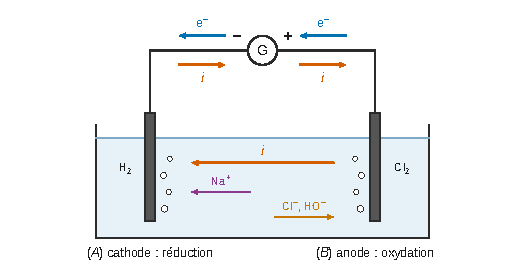
\includegraphics{figures/q8-electrolyse-sens-courant.pdf}
\caption*{Figure 1 --- figure 8 complétée : (A) cathode reliée à la borne −, (B)
anode reliée à la borne +, électrons de (B) vers (A) par les fils,
courant i en sens inverse et de (B) vers (A) dans la solution}
\end{figure}

\textbf{Q9.} Dans le sens écrit, l'oxydant qui réagit est \(\mathrm{H_2O}\) (\(E_1^\circ = -0{,}83\) V) et le réducteur est \(\mathrm{Cl^-}\) (\(E_3^\circ = 1{,}36\) V). On fait donc réagir l'oxydant le plus faible avec le réducteur le plus faible : la réaction spontanée est la réaction inverse. Quantitativement, \(\log K^\circ = 2(E_1^\circ - E_3^\circ)/0{,}06 = -73\). \textbf{L'étape 1 est thermodynamiquement très défavorisée} (\(K^\circ \approx 10^{-73}\)). C'est le générateur qui la force, d'où le nom d'électrolyse.

\hypertarget{iii.2-uxe9tude-de-luxe9tape-2}{%
\subsubsection{III.2 --- Étude de l'étape 2}\label{iii.2-uxe9tude-de-luxe9tape-2}}

\textbf{Q10.} L'étape 2 est la dismutation de \(\mathrm{Cl_2}\). On utilise les demi-équations :

\equationajustee{\begin{aligned}
(1)\quad & \tfrac12\mathrm{Cl_{2(g)}} + e^- = \mathrm{Cl^-} && (E_3^\circ = 1{,}36\ \mathrm{V}) \\
(2)\quad & \mathrm{ClO^-} + \mathrm{H_2O} + e^- = \tfrac12\mathrm{Cl_{2(g)}} + 2\,\mathrm{HO^-} && (E_4^\circ = 0{,}42\ \mathrm{V})
\end{aligned}}

\((1)-(2)\) redonne l'équation de l'étape 2, avec \(n = 1\) :

\equationajustee{\boxed{K^\circ = \frac{\dfrac{[\mathrm{Cl^-}]}{c^\circ}\,\dfrac{[\mathrm{ClO^-}]}{c^\circ}}{\dfrac{P_{\mathrm{Cl_2}}}{P^\circ}\left(\dfrac{[\mathrm{HO^-}]}{c^\circ}\right)^2}}}

À l'équilibre, les potentiels des deux couples sont égaux, d'où :

\equationajustee{\begin{aligned}
\log K^\circ &= \frac{E_3^\circ - E_4^\circ}{0{,}06} \\
&= 15{,}7
\end{aligned}}

\equationajustee{\boxed{K^\circ \approx 5\times 10^{15}}}

La réaction est quantitative.

\textbf{Q11.} Pendant \(t = 3600\) s à \(I = 20\) A :

\equationajustee{\begin{aligned}
n(e^-) &= \frac{I t}{F} \\
&= \frac{7{,}2\times 10^4}{96\,485}
\end{aligned}}

\equationajustee{\boxed{n(e^-) \simeq 0{,}75\ \mathrm{mol}}}

L'étape 1 échange 2 électrons par \(\mathrm{Cl_2}\), donc \(n(\mathrm{Cl_2}) = 0{,}37\) mol. Elle produit aussi \(n(\mathrm{HO^-}) = 0{,}75\) mol, en proportions exactement stœchiométriques pour l'étape 2, qui forme un \(\mathrm{ClO^-}\) par \(\mathrm{Cl_2}\) :

\equationajustee{\boxed{n(\mathrm{ClO^-}) \simeq 0{,}37\ \mathrm{mol\ par\ heure}}}

\textbf{Q12.} L'étape 1 consomme \(n(\mathrm{Cl^-}) = 2\,n(\mathrm{Cl_2}) = n(e^-) = 0{,}75\) mol par heure, avec \(M(\mathrm{NaCl}) = 58{,}5\ \mathrm{g\cdot mol^{-1}}\) :

\equationajustee{\boxed{m(\mathrm{NaCl}) \simeq 44\ \mathrm{g}\ \text{par heure}}}

Le bassin contient \(V = 1250\times 3 = 3{,}75\times 10^3\ \mathrm{m^3} = 3{,}75\times 10^6\) L, soit \(m_{\text{dispo}} = 5\times 3{,}75\times 10^6\ \mathrm{g} \approx 1{,}9\times 10^7\) g (19 t). \textbf{Le stock suffit pour environ \(4\times 10^5\) heures de traitement, même sans régénération.}

\hypertarget{iii.3-ajustement-du-ph}{%
\subsubsection{III.3 --- Ajustement du pH}\label{iii.3-ajustement-du-ph}}

\textbf{Q13.} Pour le couple \(\mathrm{HClO/ClO^-}\) :

\equationajustee{\frac{[\mathrm{ClO^-}]}{[\mathrm{HClO}]} = 10^{\,\mathrm{pH} - \mathrm{p}K_a}}

À pH = 8,0, ce rapport vaut \(10^{0{,}5} \approx 3{,}2\) : \(\mathrm{ClO^-}\) prédomine. L'acide sulfurique, acide fort, apporte des ions \(\mathrm{H_3O^+}\) qui réagissent totalement sur la base \(\mathrm{ClO^-}\) :

\equationajustee{\mathrm{H_3O^+} + \mathrm{ClO^-} \to \mathrm{HClO} + \mathrm{H_2O},\qquad K^\circ = 10^{7{,}5}.}

Le rapport \([\mathrm{ClO^-}]/[\mathrm{HClO}]\) diminue, donc le pH diminue aussi. Ramener le pH entre 7,2 et 7,6 revient à ramener ce rapport entre 0,50 et 1,3. \textbf{L'ajout d'acide fort convertit \(\mathrm{ClO^-}\) en \(\mathrm{HClO}\) et abaisse le pH}, ce qui favorise en outre \(\mathrm{HClO}\), la forme la plus désinfectante.

\hypertarget{partie-b-vuxe9locimuxe9trie-laser-uxe0-franges}{%
\section{Partie B --- Vélocimétrie laser à franges}\label{partie-b-vuxe9locimuxe9trie-laser-uxe0-franges}}

\hypertarget{i-expansion-du-faisceau}{%
\subsection{I --- Expansion du faisceau}\label{i-expansion-du-faisceau}}

\textbf{Q14.} Pour qu'un faisceau parallèle ressorte parallèle, le système doit être afocal : \(F'_1 \equiv F_2\), et les lentilles sont distantes de \(D = f'_1 + f'_2\). Les rayons incidents parallèles à l'axe convergent en \(F'_1\), s'y croisent, puis ressortent de \(\mathcal L_2\) parallèles à l'axe, plus écartés et inversés.

\begin{figure}[H]
\centering
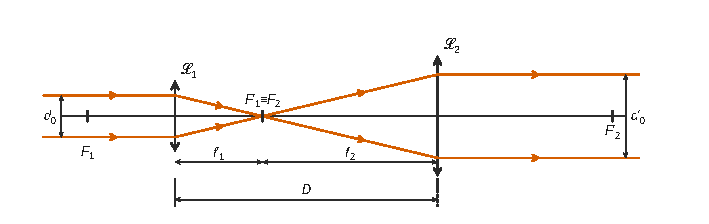
\includegraphics{figures/q14-expanseur-keplerien.pdf}
\caption*{Figure 2 --- expanseur képlérien : F′1 ≡ F2, rayons croisés en F′1,
sortie parallèle et inversée, D = f′1 + f′2 (tracé pour τ = 2)}
\end{figure}

On a \(\tau > 1\) si et seulement si \(f'_2 > f'_1\).

\textbf{Q15.} Un rayon incident à la hauteur \(h = d_0/2\) passe par \(F'_1\), puis parcourt \(f'_2\) jusqu'à \(\mathcal L_2\). Par triangles semblables, sa hauteur y vaut \(|h'| = h\,f'_2/f'_1\). D'où :

\equationajustee{\boxed{\tau = \frac{f'_2}{f'_1}}}

\textbf{Q16.} La lentille divergente \(\mathcal L_3\) (\(f'_3 < 0\)) a son foyer image \(F'_3\) \textbf{avant} elle, à \(|f'_3|\). L'afocalité impose \(F'_3 \equiv F_1\), d'où :

\equationajustee{\begin{aligned}
D &= f'_1 + f'_3 \\
&= f'_1 - |f'_3|.
\end{aligned}}

Après \(\mathcal L_3\), les rayons divergent comme s'ils venaient de \(F'_3\), puis ressortent de \(\mathcal L_1\) parallèles à l'axe, plus écartés et du même côté de l'axe : aucun point de convergence réel n'apparaît dans le système.

\begin{figure}[H]
\centering
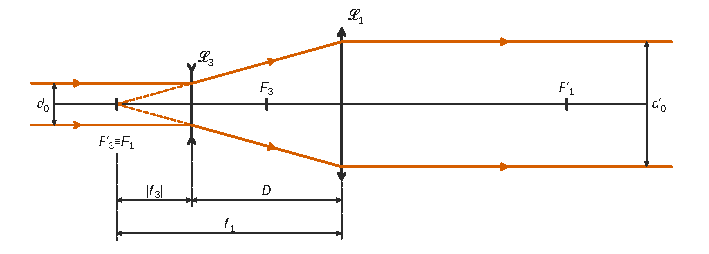
\includegraphics{figures/q16-expanseur-galileen.pdf}
\caption*{Figure 3 --- expanseur galiléen : F′3 ≡ F1 à gauche de 𝓛3, rayons
semblant venir de F′3, sortie parallèle non inversée, D = f′1 −
\textbar f′3\textbar{} (tracé pour τ′ = 3)}
\end{figure}

\textbf{Q17.} Après \(\mathcal L_3\), le rayon de hauteur \(h\) semble issu de \(F'_3 \equiv F_1\). Il atteint \(\mathcal L_1\), située à \(f'_1\) de ce point, à la hauteur \(h\,f'_1/|f'_3|\) :

\equationajustee{\boxed{\tau' = \frac{f'_1}{|f'_3|} = -\frac{f'_1}{f'_3}}}

\textbf{Q18.} Pour le montage képlérien, \(f'_2 = \tau f'_1\). Pour le montage galiléen, \(f'_3 = -f'_1/\tau'\). D'où :

\equationajustee{\boxed{D_{\text{kep}} = f'_1(1+\tau)}}

\equationajustee{\boxed{D_{\text{gal}} = f'_1\left(1 - \frac{1}{\tau'}\right)}}

À \(f'_1\) et taux \(\tau = \tau' > 1\) égaux, \(D_{\text{gal}} < f'_1 < D_{\text{kep}}\). Par exemple, pour \(\tau = 3\) : \(0{,}67 f'_1\) contre \(4 f'_1\). \textbf{L'expanseur galiléen est le plus compact.}

\hypertarget{ii-division-du-faisceau}{%
\subsection{II --- Division du faisceau}\label{ii-division-du-faisceau}}

\textbf{Q19.} Le cube est vu en coupe comme un carré de côté \(c\), dont une diagonale porte l'axe. Les rayons incidents arrivent donc sur les faces de gauche sous \(i = 45^\circ\). La loi de Snell-Descartes donne :

\equationajustee{\begin{aligned}
\sin r &= \frac{\sin 45^\circ}{1{,}5} \\
&= 0{,}471, \\
r &= 28{,}1^\circ.
\end{aligned}}

\begin{itemize}
\tightlist
\item
  \textbf{Rayon supérieur.} Il est réfracté par la face supérieure gauche et dévié de \(16{,}9^\circ\) vers le bas. Il atteint la face inférieure droite, \textbf{parallèle} à la face d'entrée, sous l'incidence \(r\), et ressort sous \(45^\circ\) : il émerge parallèle à l'axe, translaté vers le bas de \(c\,\sin(i-r)/\cos r \approx 0{,}33\,c\), donc \textbf{sous l'axe}.
\item
  \textbf{Rayon inférieur.} Par symétrie, il est dévié vers le haut et ressort parallèle à l'axe, \textbf{au-dessus de l'axe}.
\item
  \textbf{Rayon axial.} Il frappe l'arête gauche et est partagé entre les deux faces de gauche. Sa partie réfractée par la face supérieure ressort à \(0{,}33\,c\) sous l'axe, celle réfractée par la face inférieure à \(0{,}33\,c\) au-dessus.
\end{itemize}

\begin{figure}[H]
\centering
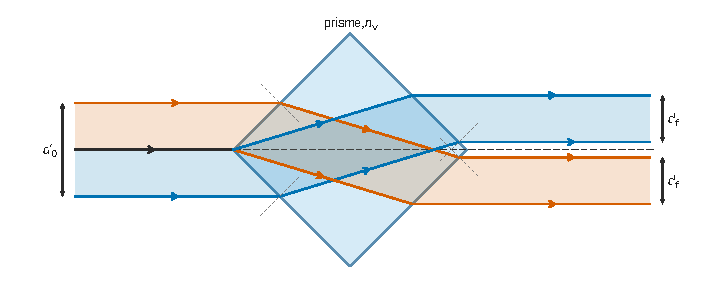
\includegraphics{figures/q19-prisme-division-faisceau.pdf}
\caption*{Figure 4 --- prisme cubique : chaque moitié du faisceau (orange, bleue)
traverse une lame à faces parallèles et ressort parallèle à l'axe, de
l'autre côté, d'où d\_f = d′0/2}
\end{figure}

Le faisceau est donc divisé par l'arête en deux demi-faisceaux. Chacun traverse une lame à faces parallèles : il ressort parallèle à l'axe, et les deux demi-faisceaux se sont croisés dans le prisme. Ce tracé suppose \(d'_0 < 0{,}66\,c\). Un rayon entrant plus haut atteindrait la face supérieure droite sous \(61{,}9^\circ > \arcsin(1/1{,}5) = 41{,}8^\circ\) et y subirait une réflexion totale.

\textbf{Q20.} L'arête coupe le faisceau en deux moitiés égales. Une lame à faces parallèles translate un faisceau sans changer sa largeur (les facteurs \(\cos r/\cos i\) des deux dioptres se compensent). D'où :

\equationajustee{\boxed{d_f = \frac{d'_0}{2}}}

\textbf{Q21.} Dans chaque demi-faisceau, l'onde reste plane : par le théorème de Malus, les plans orthogonaux à l'axe sont des surfaces d'onde. Le dispositif est symétrique par rapport à l'axe, donc deux rayons symétriques ont le même chemin optique. Un plan orthogonal à l'axe en sortie est ainsi une surface d'onde commune aux deux faisceaux :

\equationajustee{\boxed{\delta = 0}}

Les deux faisceaux sont plans, de même intensité (division en deux moitiés égales), issus de la même source et en phase. \textbf{Ils remplissent les conditions de cohérence et d'égalité d'intensité requises, quelle que soit la longueur de cohérence du laser.}

\hypertarget{iii-interfuxe9rences-des-deux-faisceaux}{%
\subsection{III --- Interférences des deux faisceaux}\label{iii-interfuxe9rences-des-deux-faisceaux}}

\textbf{Q22.} D'après la figure 12, avec \(k = 2\pi/\lambda_0\) :

\equationajustee{\begin{aligned}
\vec k_1 &= k(\cos\alpha\,\vec u_x - \sin\alpha\,\vec u_y), \\
\vec k_2 &= k(\cos\alpha\,\vec u_x + \sin\alpha\,\vec u_y), \\
\vec k_2 - \vec k_1 &= 2k\sin\alpha\,\vec u_y .
\end{aligned}}

Comme \(I \propto |\underline s_1 + \underline s_2|^2\) et que chaque onde seule donne \(I_0\) :

\equationajustee{\boxed{I(x,y,z) = 2I_0\left[1 + \cos\left(\frac{4\pi\sin\alpha}{\lambda_0}\,y\right)\right]}}

\(I\) ne dépend que de \(y\). Dans la zone de recouvrement, on observe des franges rectilignes, parallèles à \((Ox)\) : ce sont des plans \(y =\) cte.

Elles sont équidistantes, de contraste maximal (\(I\) varie de \(0\) à \(4I_0\)), avec une frange brillante en \(y = 0\).

\textbf{Q23.} L'interfrange est la distance entre deux franges brillantes consécutives, mesurée perpendiculairement aux franges (ici selon \(y\)) :

\equationajustee{\boxed{i = \frac{\lambda_0}{2\sin\alpha}}}

\equationajustee{\begin{aligned}
i &= \frac{514\times 10^{-9}}{2\times 0{,}1045} \\
&= 2{,}46\ \mathrm{\mu m}.
\end{aligned}}

\textbf{Q24.} Une particule se déplaçant selon \(y\) à la vitesse \(V\) franchit un interfrange par période de clignotement, donc \(f = V/i\) :

\equationajustee{\boxed{V = \frac{\lambda_0 f}{2\sin\alpha}}}

\equationajustee{\begin{aligned}
V &= \frac{514\times 10^{-9}\times 1{,}200\times 10^6}{0{,}2091} \\
&= 2{,}95\ \mathrm{m\cdot s^{-1}}.
\end{aligned}}

Pour l'incertitude, la formule produit/quotient s'applique. L'incertitude relative sur \(\sin\alpha\) vaut :

\equationajustee{\begin{aligned}
\frac{u(\sin\alpha)}{\sin\alpha} &= \frac{u(\alpha)}{\tan\alpha} \\
&= \frac{1{,}745\times 10^{-3}}{0{,}1051} \\
&= 1{,}66\ \%.
\end{aligned}}

On compose avec \(u(\lambda_0)/\lambda_0 = 1{,}95\ \%\) et \(u(f)/f = 4{,}17\ \%\) :

\equationajustee{\begin{aligned}
\frac{u(V)}{V} &= \sqrt{(1{,}95\ \%)^2 + (4{,}17\ \%)^2 + (1{,}66\ \%)^2} \\
&= 4{,}9\ \%.
\end{aligned}}

\equationajustee{\boxed{V = (2{,}95 \pm 0{,}14)\ \mathrm{m\cdot s^{-1}}}}

\textbf{Q25.} Le faisceau 1 occupe la bande \(|x\sin\alpha + y\cos\alpha| \le d_f/2\), le faisceau 2 la bande \(|x\sin\alpha - y\cos\alpha| \le d_f/2\). La zone commune est un losange. Sur \((Oy)\), la condition s'écrit \(|y| \le d_f/(2\cos\alpha)\), d'où :

\equationajustee{\boxed{\Delta = \frac{d_f}{\cos\alpha}}}

\textbf{Q26.} Pour qu'une particule clignote au moins deux fois, ce qui est nécessaire pour définir une fréquence, elle doit traverser au moins un interfrange dans la zone : \(\Delta \ge i\). D'où :

\equationajustee{\frac{d_f}{\cos\alpha} \ge \frac{\lambda_0}{2\sin\alpha}}

\equationajustee{\boxed{d_{f,\min} = \frac{\lambda_0}{2\tan\alpha} \approx 2{,}4\ \mathrm{\mu m}}}

Le laser fournit \(d_f = 0{,}65\) mm, soit environ 270 fois plus. La zone contient \(N = \Delta/i = 2 d_f\tan\alpha/\lambda_0 \approx 2{,}7\times 10^2\) franges. Si l'on interprète 0,65 mm comme le diamètre en sortie du laser, avant expansion et division, \(d_f \ge 0{,}33\) mm et \(N \gtrsim 130\). \textbf{Le laser argon convient largement} : chaque particule produit une centaine d'éclats, ce qui permet une mesure précise de la fréquence.

\hypertarget{partie-c-le-plongeon-de-haut-vol}{%
\section{Partie C --- Le plongeon de haut vol}\label{partie-c-le-plongeon-de-haut-vol}}

\textbf{Q27.} On étudie le plongeur entièrement immergé, de volume \(V = m/\rho_h\), dans le référentiel du bassin supposé galiléen, avec un axe vertical \textbf{descendant} et \(v > 0\). Il subit son poids \(mg\), la poussée d'Archimède \(-\rho\,\dfrac{m}{\rho_h}\,g\) et la traînée \(-kv^2\). La deuxième loi de Newton donne :

\equationajustee{\boxed{\frac{\mathrm dv}{\mathrm dt} = g\left(1 - \frac{\rho}{\rho_h}\right) - \frac{k}{m}\,v^2}}

\textbf{Q28.} On pose \(\varphi(v) = B - A v^2\), avec :

\equationajustee{\begin{aligned}
A &= \frac{k}{m} > 0, \\
B &= g\left(1-\frac{\rho}{\rho_h}\right) > 0 \quad (\text{car } \rho_h > \rho).
\end{aligned}}

La fonction \(\varphi\) décroît strictement sur \(\mathbb R_+\) et s'annule en une unique valeur :

\equationajustee{\boxed{v_{\text{lim}} = \sqrt{\frac{m g}{k}\left(1 - \frac{\rho}{\rho_h}\right)} = \sqrt{\frac{2 m g(\rho_h - \rho)}{\rho_h\,\rho\, C_x S}}}}

La constante \(v_{\text{lim}}\) est solution. Par unicité (Cauchy-Lipschitz), une solution partie de \(v_0 > v_{\text{lim}}\) reste au-dessus de \(v_{\text{lim}}\).

Elle est alors décroissante, puisque \(\varphi < 0\), et minorée, donc elle converge vers une limite \(\ell\) qui doit vérifier \(\varphi(\ell) = 0\) : \(\ell = v_{\text{lim}}\).

\emph{Estimations.}
- \textbf{\(C_x\)} : le plongeur gainé, bras tendus, s'apparente à un cylindre allongé (\(L/D \approx 5\)). Le tableau 2 donne \(C_x = 0{,}35\) aux grandes vitesses, ce qui convient pendant la phase de freinage. Aux faibles vitesses, les valeurs voisines (0,47 à 0,74) changeraient \(v_{\text{lim}}\) d'environ 30 \% au plus.
- \textbf{\(S\)} : la figure 14 n'a pas d'échelle. Une section de corps humain vaut entre 0,1 m² (entrée parfaitement verticale) et 0,3 m² (corps légèrement incliné, bras et jambes compris). On retient \(S \approx 0{,}3\) m², valeur cohérente avec la figure 15.

On obtient \(k = \tfrac12\times 1000\times 0{,}35\times 0{,}30 \approx 53\ \mathrm{kg\cdot m^{-1}}\) et \(m g(1-\rho/\rho_h) = 75\times 9{,}81\times 0{,}0706 = 52\) N, d'où :

\equationajustee{\boxed{v_{\text{lim}} \approx 1{,}0\ \mathrm{m\cdot s^{-1}}}}

Avec \(S = 0{,}1\) m², on trouverait 1,7 m/s. La valeur est faible parce que la poussée d'Archimède compense 93 \% du poids. Elle concorde avec l'asymptote de la figure 15 pour \(C_x = 0{,}35\).

\textbf{Q29.} Par identification avec Q27 :

\equationajustee{\boxed{A = \frac{k}{m}}}

\equationajustee{\boxed{B = g\left(1 - \frac{\rho}{\rho_h}\right)}}

On pose \(u = e^{-2t/\tau + k_2}\), de sorte que \(v = k_1\dfrac{1+u}{1-u}\) et \(\dot u = -\dfrac{2u}{\tau}\). Alors :

\equationajustee{\begin{aligned}
\frac{\mathrm dv}{\mathrm dt} &= -\frac{4k_1 u}{\tau(1-u)^2}, \\
-A v^2 + B &= \frac{-A k_1^2 (1+u)^2 + B(1-u)^2}{(1-u)^2}.
\end{aligned}}

L'identification pour tout \(t\) impose \(A k_1^2 = B\). Le second membre vaut alors \(-4Bu/(1-u)^2\), et il faut \(k_1/\tau = B\).

Enfin, \(v(0) = v_0\) donne \(e^{k_2} = (v_0 - k_1)/(v_0 + k_1)\) :

\equationajustee{\boxed{\begin{aligned}
k_1 &= \sqrt{\frac{B}{A}} = v_{\text{lim}} \\
\tau &= \frac{1}{\sqrt{AB}} \\
k_2 &= \ln\left(\frac{v_0 - \sqrt{B/A}}{v_0 + \sqrt{B/A}}\right) < 0
\end{aligned}}}

Numériquement, on prend \(A \approx 0{,}70\ \mathrm{m^{-1}}\), \(B = 0{,}69\ \mathrm{m\cdot s^{-2}}\) et \(v_0 = 13{,}9\ \mathrm{m\cdot s^{-1}}\). On obtient \(k_1 \approx 1{,}0\ \mathrm{m\cdot s^{-1}}\), \(\tau \approx 1{,}4\) s et \(k_2 \approx -0{,}14\).

\textbf{Q30.} \emph{Principe de la méthode d'Euler.} On discrétise \([t_0, t_f]\) avec le pas \(h\) et l'on remplace la dérivée par un taux d'accroissement. Le développement à l'ordre 1 donne la récurrence :

\equationajustee{v(t_{i+1}) \simeq v(t_i) + h\,F(v(t_i))}

Elle permet de construire la solution de proche en proche à partir de \(v(t_0) = v_0\). L'erreur globale est en \(O(h)\), et le pas doit rester petit devant \(\tau\) (ici \(h = 10^{-2}\) s pour \(\tau \approx 1{,}4\) s).

\begin{lstlisting}[language=Python]
    return -A*v**2 + B                                    # ligne 6
        valeurs_v.append(valeurs_v[i] + h*F(valeurs_v[i]))  # ligne 14
\end{lstlisting}

Exécuté avec \(A = 0{,}70\), \(B = 0{,}69\) et \(v_0 = 13{,}9\), ce programme donne \(v(10\ \mathrm s) = 0{,}99\ \mathrm{m\cdot s^{-1}}\), en accord avec la solution analytique.

\textbf{Q31.} Le temps de réaction vaut 1 s. Pour un corps humain à grande vitesse, le coefficient réaliste est \(C_x = 0{,}35\) (cylindre, \(L/D \approx 5\)) ou \(0{,}47\). À \(t = 1\) s, la figure 15 donne :
- pour \(C_x = 0{,}35\) : \(z_G \approx -3{,}5\) m et \(v \approx 1{,}5\ \mathrm{m\cdot s^{-1}}\) ;
- pour \(C_x = 0{,}47\) : \(z_G \approx -3\) m.

Les mains, tendues 1 m sous le centre de masse, sont alors à environ \(-4{,}5\) m. \textbf{Un bassin de 5 m laisse donc au plongeur le temps de réagir} (ouvrir les bras, se cambrer, remonter) avant de toucher le fond. À cet instant, sa vitesse est déjà faible. À l'inverse, une position parfaitement profilée (\(C_x = 0{,}04\)) donnerait \(z_G \approx -10\) m dès la première seconde : le plongeur doit rompre l'alignement dès l'entrée. Dans un bassin de 3 m, les mains toucheraient le fond (\(z_G = -2\) m) au bout de 0,3 s seulement, à environ 3,6 m/s.

\hypertarget{partie-d-comment-uxe9viter-lhypothermie-en-natation-marathon-ou-triathlon}{%
\section{Partie D --- Comment éviter l'hypothermie en natation marathon ou triathlon ?}\label{partie-d-comment-uxe9viter-lhypothermie-en-natation-marathon-ou-triathlon}}

\textbf{Q32.} On considère une couche plane d'épaisseur \(e_e\), de section \(S\), en régime stationnaire et sans source. Le bilan sur une tranche \([x, x+\mathrm dx]\) montre que le flux \(\Phi = j\,S\) est uniforme. La loi de Fourier \(j = -\lambda_e\,\mathrm dT/\mathrm dx\) s'intègre alors en \(T_1 - T_2 = \Phi\,e_e/(\lambda_e S)\) :

\equationajustee{\boxed{R_e = \frac{e_e}{\lambda_e S}}}

Les trois couches sont traversées par le même flux : elles sont en série.

\equationajustee{\boxed{R_{\text{peau}} = \frac{1}{S}\left(\frac{e_e}{\lambda_e} + \frac{e_d}{\lambda_d} + \frac{e_g}{\lambda_g}\right)}}

On calcule \(S = 0{,}007184\times 75^{0{,}425}\times 175^{0{,}725} = 1{,}90\ \mathrm{m^2}\). Les trois termes de la parenthèse valent, en \(\mathrm{m^2\cdot K\cdot W^{-1}}\) :

\equationajustee{\begin{aligned}
\frac{e_e}{\lambda_e} &= 3{,}3\times 10^{-4}, \\
\frac{e_d}{\lambda_d} &= 4{,}4\times 10^{-3}, \\
\frac{e_g}{\lambda_g} &= 5{,}26\times 10^{-2}.
\end{aligned}}

Leur somme vaut \(5{,}74\times 10^{-2}\), d'où :

\equationajustee{\boxed{R_{\text{peau}} \approx 3{,}0\times 10^{-2}\ \mathrm{K\cdot W^{-1}}}}

La graisse en fournit 92 \%.

\textbf{Q33.} Le flux conducto-convectif vaut \(\Phi_{cc} = h S\,(T_{\text{paroi}} - T_0)\), d'où :

\equationajustee{\boxed{R_{cc} = \frac{1}{hS} = \frac{1}{455{,}0\times 1{,}90} \approx 1{,}2\times 10^{-3}\ \mathrm{K\cdot W^{-1}}}}

\textbf{Q34.} On factorise \(T_{\text{paroi}}^4 - T_0^4 = (T_{\text{paroi}}^2 + T_0^2)(T_{\text{paroi}} + T_0)\,\Delta T\). Pour \(\Delta T \ll T_0\), cela donne \(\simeq 4T_0^3\,\Delta T\), d'où \(\Phi_{\text{rad}} \simeq 4\varepsilon\sigma S T_0^3\,\Delta T\), proportionnel à \(\Delta T\). Avec \(T_0 = 289\) K :

\equationajustee{\boxed{R_{\text{rad}} = \frac{1}{4\varepsilon\sigma S T_0^3}}}

\equationajustee{R_{\text{rad}} = \frac{1}{4\times 0{,}9\times 5{,}7\times 10^{-8}\times 1{,}90\times 289^3}}

\equationajustee{\boxed{R_{\text{rad}} \approx 0{,}11\ \mathrm{K\cdot W^{-1}}}}

\textbf{Q35.} La chaleur traverse successivement la peau et la combinaison (même flux, donc en série). Depuis la paroi externe, à \(T_{\text{paroi}}\), elle rejoint l'eau par deux voies soumises au même écart \(T_{\text{paroi}} - T_0\) : convection et rayonnement, en parallèle.

\begin{figure}[H]
\centering
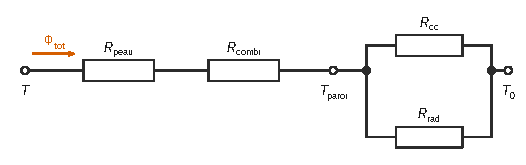
\includegraphics{figures/q35-schema-resistances-thermiques.pdf}
\caption*{Figure 5 --- schéma équivalent : R\_peau et R\_combi en série, puis
R\_cc et R\_rad en parallèle entre T\_paroi et T\_0}
\end{figure}

\equationajustee{\boxed{R_{\text{tot}} = R_{\text{peau}} + R_{\text{combi}} + \frac{R_{cc}\,R_{\text{rad}}}{R_{cc} + R_{\text{rad}}}}}

\equationajustee{\boxed{\Phi_{\text{tot}} = \frac{T - T_0}{R_{\text{tot}}}}}

\textbf{Q36.} On compare les deux branches parallèles : \(R_{\text{rad}}/R_{cc} \approx 0{,}106/1{,}15\times 10^{-3} \approx 92\). L'association parallèle vaut alors :

\equationajustee{\frac{R_{cc}}{1 + R_{cc}/R_{\text{rad}}} = 0{,}989\,R_{cc}}

\textbf{Le rayonnement est négligeable devant la convection dans l'eau}, car \(h = 455\ \mathrm{W\cdot m^{-2}\cdot K^{-1}}\) est très supérieur au coefficient radiatif équivalent \(4\varepsilon\sigma T_0^3 \approx 5\ \mathrm{W\cdot m^{-2}\cdot K^{-1}}\).

La résistance de la combinaison vaut :

\equationajustee{\begin{aligned}
R_{\text{combi}} &= \frac{e}{\lambda_{\text{Ar}} S} \\
&= \frac{4{,}0\times 10^{-3}}{0{,}04887\times 1{,}90} \\
&= 4{,}3\times 10^{-2}\ \mathrm{K\cdot W^{-1}}.
\end{aligned}}

D'où :

\equationajustee{\begin{aligned}
R_{\text{tot}} &\simeq R_{\text{peau}} + R_{\text{combi}} + R_{cc} \\
&= 3{,}02\times 10^{-2} + 4{,}30\times 10^{-2} + 0{,}12\times 10^{-2}
\end{aligned}}

\equationajustee{\boxed{R_{\text{tot}} \approx 7{,}4\times 10^{-2}\ \mathrm{K\cdot W^{-1}}}}

La combinaison représente 58 \% de la résistance totale, et \(R_{cc}\) est elle-même presque négligeable (1,6 \%).

\textbf{Q37.} On applique le premier principe au nageur, de capacité \(mc\) et de température uniforme, le régime étant lentement variable :

\equationajustee{mc\,\frac{\mathrm dT}{\mathrm dt} = \mathcal P_h - \frac{T - T_0}{R_{\text{tot}}}}

En divisant par \(mc\), on obtient la forme demandée :

\equationajustee{\frac{\mathrm dT}{\mathrm dt} + \frac{T}{\tau} = \xi}

\equationajustee{\boxed{\begin{aligned}
\tau &= m c R_{\text{tot}} \\
\xi &= \frac{\mathcal P_h}{mc} + \frac{T_0}{m c R_{\text{tot}}}
\end{aligned}}}

Numériquement, \(\tau = 75\times 3{,}5\times 10^3\times 7{,}43\times 10^{-2} \approx 1{,}95\times 10^4\) s, soit 5,4 h.

\textbf{Q38.} La solution est la somme d'une solution particulière constante \(\xi\tau\) et de la solution homogène \(K e^{-t/\tau}\). Le nageur entre dans l'eau à \(T(0) = T_c\) :

\equationajustee{\boxed{T(t) = \xi\tau + (T_c - \xi\tau)\,e^{-t/\tau}}}

\textbf{Q39.} En régime permanent, \(\mathrm dT/\mathrm dt = 0\) :

\equationajustee{\boxed{T_\infty = \xi\tau = T_0 + R_{\text{tot}}\,\mathcal P_h}}

\equationajustee{T_\infty = 16{,}0 + 7{,}43\times 10^{-2}\times 250}

\equationajustee{\boxed{T_\infty \approx 34{,}6\ ^\circ\mathrm C}}

Le régime permanent est atteint à 1 \% près au bout d'environ \(5\tau\) : \(\boxed{t \approx 5\tau \approx 1\times 10^5\ \mathrm s \approx 27\ \mathrm h}\). On note que \(T_\infty < 35\ ^\circ\)C.

\textbf{Q40.} De \(T(t) = T_\infty + (T_c - T_\infty)\,e^{-t/\tau}\), on tire :

\equationajustee{\boxed{t_{\text{max}} = \tau\ln\frac{T_c - T_\infty}{35 - T_\infty}}\qquad(\text{\text{défini} si } T_\infty < 35\ ^\circ\mathrm C).}

\begin{itemize}
\tightlist
\item
  \textbf{Avec combinaison} : \(R_{\text{tot}} = R_{\text{peau}} + R_{\text{combi}} + R_{cc} = 7{,}43\times 10^{-2}\ \mathrm{K\cdot W^{-1}}\), \(\tau = 1{,}95\times 10^4\) s et \(T_\infty = 34{,}58\ ^\circ\)C. D'où \(t_{\text{max}} = 1{,}95\times 10^4\,\ln(2{,}42/0{,}42) \approx 3{,}4\times 10^4\) s : \(\boxed{t_{\text{max}} \approx 9{,}5\ \mathrm h}\).
\item
  \textbf{Sans combinaison} : \(R'_{\text{tot}} = R_{\text{peau}} + R_{cc} = 3{,}13\times 10^{-2}\ \mathrm{K\cdot W^{-1}}\), \(\tau' = 8{,}2\times 10^3\) s et \(T'_\infty = 23{,}8\ ^\circ\)C. D'où \(t'_{\text{max}} = 8{,}2\times 10^3\,\ln(13{,}2/11{,}2) \approx 1{,}35\times 10^3\) s : \(\boxed{t'_{\text{max}} \approx 23\ \mathrm{min}}\).
\end{itemize}

Le marathon dure un peu plus de deux heures. Sans combinaison, le nageur serait en hypothermie avant la fin de la première demi-heure. Avec combinaison, il finit l'épreuve vers 36 °C, loin du seuil. \textbf{La combinaison est indispensable dans une eau à 16 °C}, ce qui justifie son caractère obligatoire.

\end{document}
